%----------------------------------------------------------------------------------------
%	PACKAGES AND THEMES
%----------------------------------------------------------------------------------------

\documentclass{beamer}

\mode<presentation> 

\usetheme{Madrid}
\usecolortheme{dolphin}
\usefonttheme{professionalfonts}

\setbeamertemplate{navigation symbols}{} 

\setbeamertemplate{sections/subsections in toc}[circle]

\setbeamertemplate{bibliography item}[triangle]

\setbeamertemplate{footline}
{
\leavevmode%
\hbox{%
    \begin{beamercolorbox}[wd=.333333\paperwidth,ht=2.25ex,dp=1ex,center]{section in head/foot}%
        \usebeamerfont{author in head/foot}\insertshortauthor \ {(\insertshortinstitute)}
    \end{beamercolorbox}%
    \begin{beamercolorbox}[wd=.333333\paperwidth,ht=2.25ex,dp=1ex,center]{section in head/foot}%
        \usebeamerfont{title in head/foot}\insertshorttitle
    \end{beamercolorbox}%
    \begin{beamercolorbox}[wd=.333333\paperwidth,ht=2.25ex,dp=1ex,right]{section in head/foot}%
        \usebeamerfont{date in head/foot}\insertshortdate{}\hspace*{2em}
    \end{beamercolorbox}}%
    \vskip0pt%
}

\setbeamertemplate{frametitle}
{
    \begin{beamercolorbox}[sep=0.3cm,ht=1.8em,wd=\paperwidth]{frametitle}
        \vbox{}\vskip-0.0ex%
        \strut\insertframetitle\strut
        \hfill
        
\includegraphics[height=1.8em,keepaspectratio]{Images/TAMU_logo_box.png}
        \vskip-2.8ex%
    \end{beamercolorbox}
}

\definecolor{maroon}{RGB}{80,0,0}

\setbeamercolor{title}{bg=maroon, fg=white}
\setbeamercolor{block title}{bg=maroon, fg=white}
\setbeamercolor{block body}{bg=maroon!05, fg=black}
\setbeamercolor{frametitle}{fg=maroon, bg=white}
\setbeamercolor{item}{fg=maroon}
\setbeamercolor{section in head/foot}{bg=maroon, fg=white}


\usepackage{graphicx}
\usepackage{booktabs}
\usepackage{textpos} 
\usepackage{media9}
\usepackage{natbib}

%----------------------------------------------------------------------------------------
%	TITLE PAGE
%----------------------------------------------------------------------------------------

\title[OSA News]{Strontium Optical Lattice Clock Comparison Over 1415 Kilometers} 

\author[J. Becker]{Joe Becker}

\institute[Texas A\&M]{Texas A\&M Department of Physics and Astronomy

\medskip
\textit{jbecker@physics.tamu.edu} % Your email address
}

\date{September 15, 2016} % Date, can be changed to a custom date

\titlegraphic{
\includegraphics[height=1.5cm]{Images/TAMU_logo.png}}

%----------------------------------------------------------------------------------------
% PRESENTATION SLIDES
%----------------------------------------------------------------------------------------

\begin{document}
\setbeamertemplate{items}[circle]

\begin{frame}
\titlepage 
\end{frame}

\begin{frame}{Outline}
    \tableofcontents
\end{frame}

\section{Motivation} 
\begin{frame}\frametitle{Why Compare Clocks?}
    \begin{block}{Moving to an Optical Standard}
        \begin{itemize}
            \item You can only measure frequency against a standard.
            \item The current time standard (caesium) is based on microwave frequencies.
            \item Current optical clock comparisons are limited to $4\times10^{-16}$ fractional agreement due to the caesium clocks. 
            \item In order to move to the new more accurate time standard optical clocks need to be directly compared.
        \end{itemize}
    \end{block}
\end{frame}

\begin{frame}\frametitle{Why Compare Clocks?}
    \begin{block}{An Optical Clock Network for New Physics}
        An optical clock network has the potential to open new avenues to experiments:
        \begin{itemize}
            \item The search for dark matter
            \item The Einstein equivalence principle 
            \item Very long baseline interferometry
            \item Building a new geodetic reference frame on relativistic geodesy
        \end{itemize}
    \end{block}
\end{frame}

\section{Background} 
\begin{frame}\frametitle{Strontium Optical Lattice Clocks}
    \begin{columns}
        \column{0.45\textwidth}
        \begin{block}{Sr Clock Schematic}
            \centering
            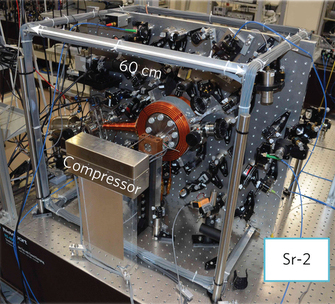
\includegraphics[width=0.5\textwidth,keepaspectratio]{Images/Sr_Clock_Img.jpg}

            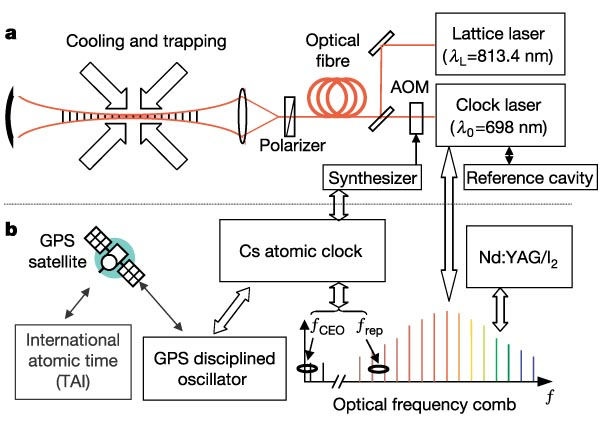
\includegraphics[width=1.0\textwidth,keepaspectratio]{Images/Sr_Clock_Schem.jpg}
        \end{block}

        \column{0.45\textwidth}
        \begin{block}{Sr Clock Lattice and Transitions}
            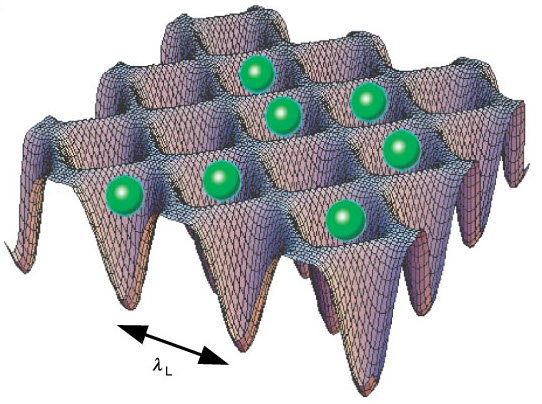
\includegraphics[width=1.0\textwidth,keepaspectratio]{Images/Sr_Clock_Lattice.jpg}

            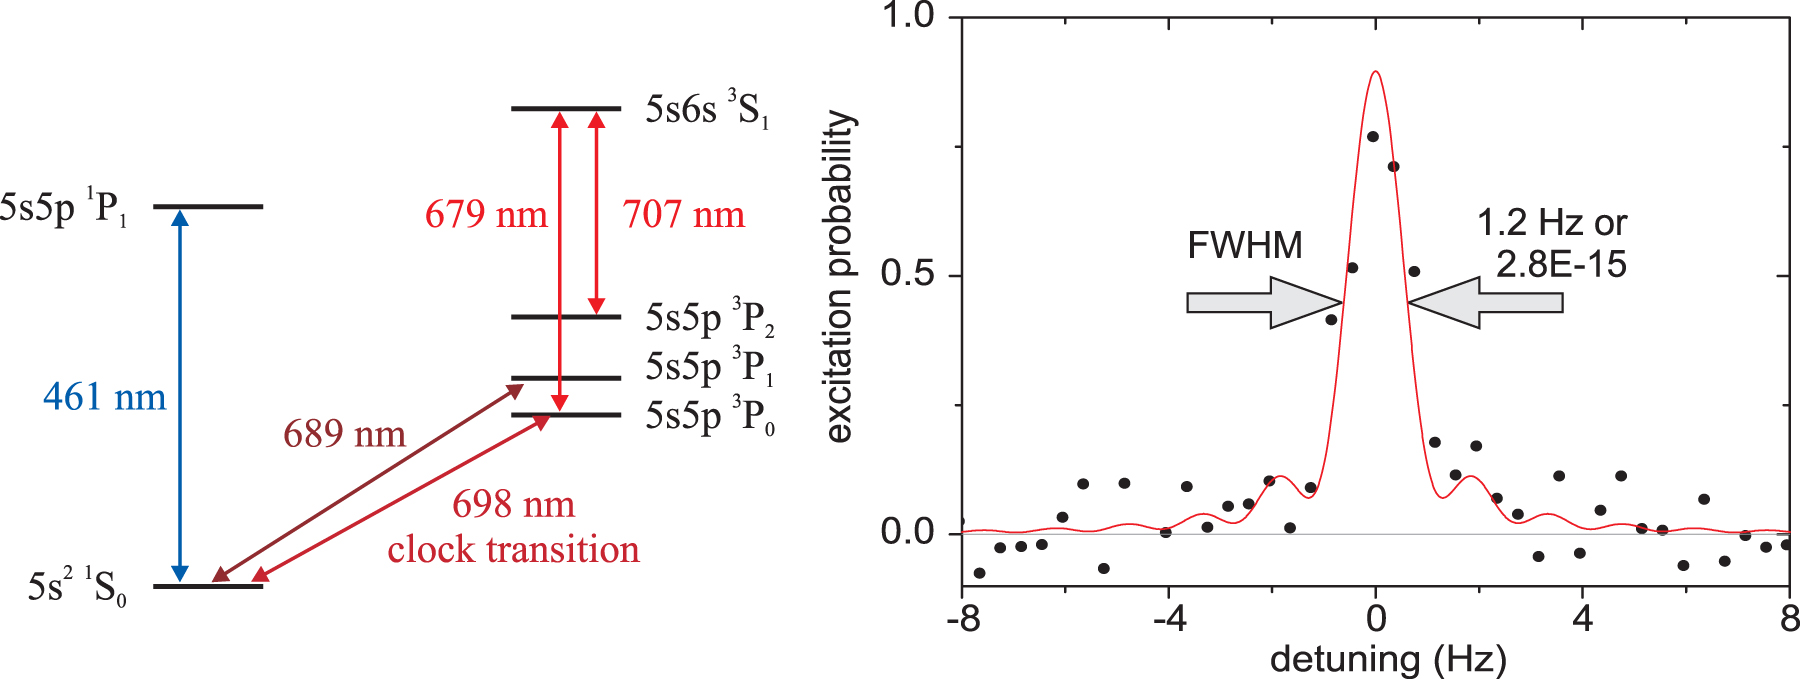
\includegraphics[width=1.0\textwidth,keepaspectratio]{Images/Sr_Trans.jpg}
        \end{block}
    \end{columns}

    \cite{Falke2014,Ushijima2015,Takamoto2005}
\end{frame}

\begin{frame}\frametitle{Strontium Clocks Frequency Comparison}
    \begin{center}
        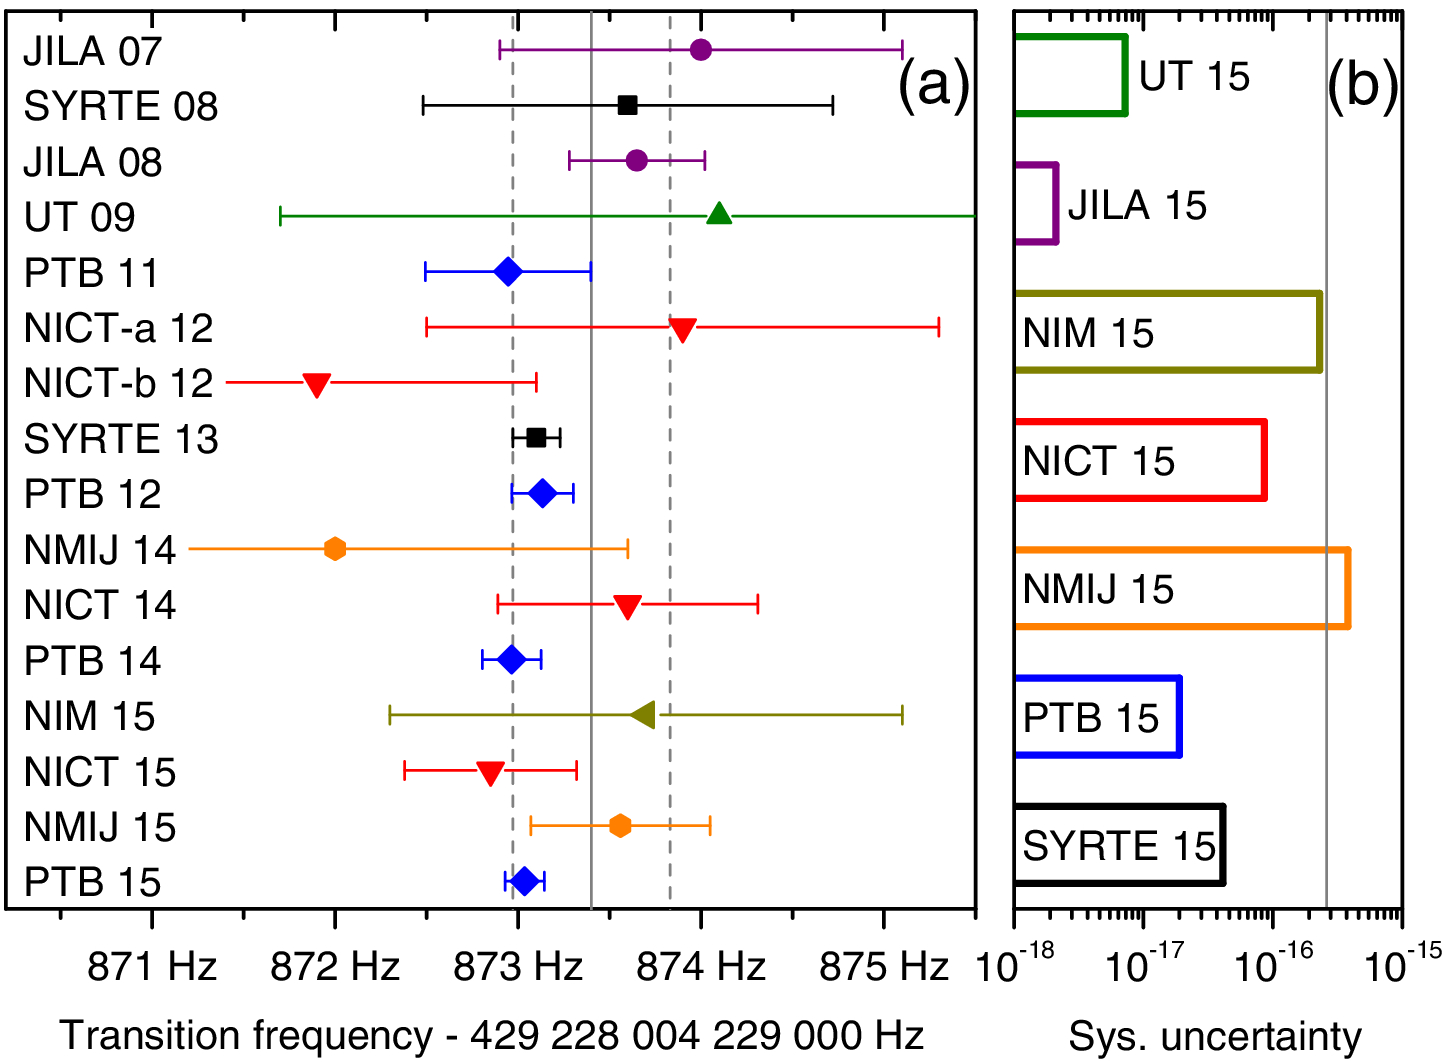
\includegraphics[width=0.8\textwidth,keepaspectratio]{Images/Sr_Clock_Comp.jpg}
    \end{center}

    \cite{Grebing2016}
\end{frame}

\section{Apparatus} 

\begin{frame}\frametitle{Schematic of Clock Comparison}
    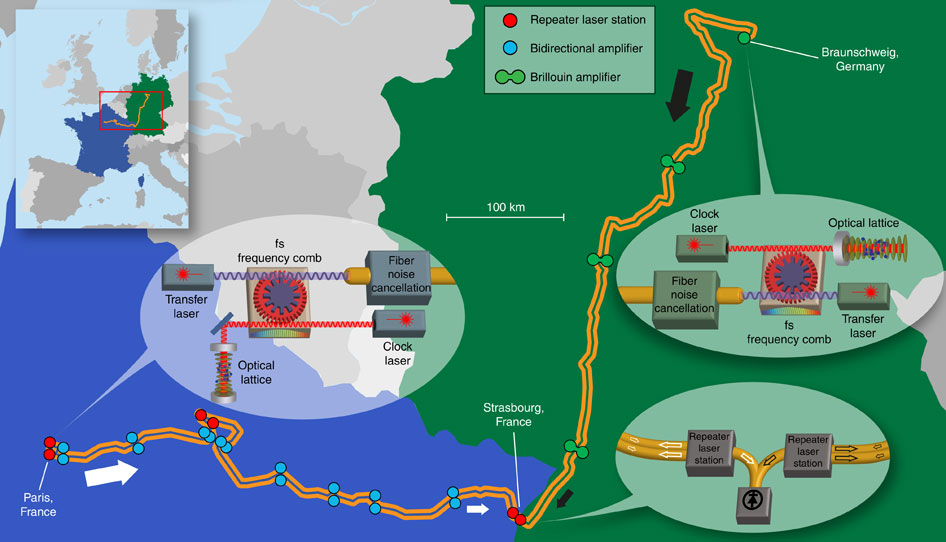
\includegraphics[width=1.0\textwidth,keepaspectratio]{Images/Link_Map.jpg}

    \cite{Lisdat2016}
\end{frame}

\begin{frame}\frametitle{Schematic of Transfer Laser System}
    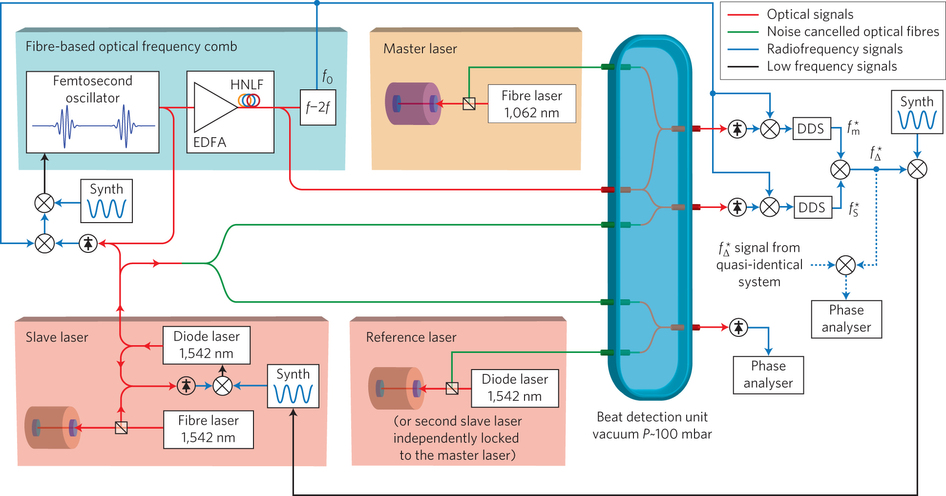
\includegraphics[width=1.0\textwidth,keepaspectratio]{Images/Transfer_Schematic.jpg}
    
    \cite{Nicolodi2014}
\end{frame}

\begin{frame}\frametitle{Braunschweig to Strasbourg Uplink}
    \begin{block}{Fiber Brillouin Amplification Schematic}
        \centering
        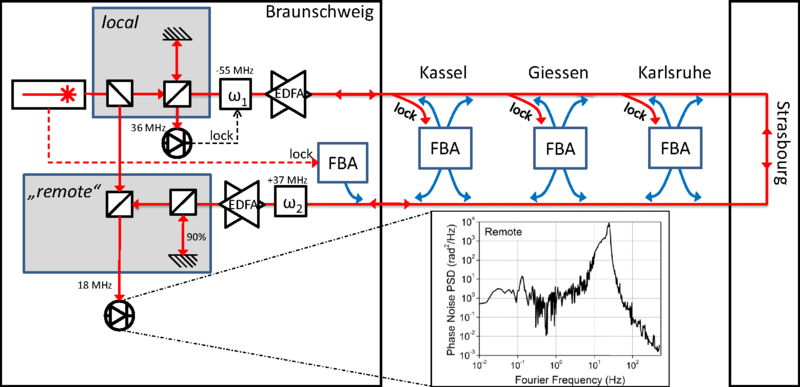
\includegraphics[width=1.0\textwidth,keepaspectratio]{Images/PTB_Loop_Schem.png}
    \end{block}
    
    \cite{Raupach2015}
\end{frame}

\begin{frame}\frametitle{Paris to Strasbourg Uplink}
    \begin{block}{Uplink Map}
        \centering
        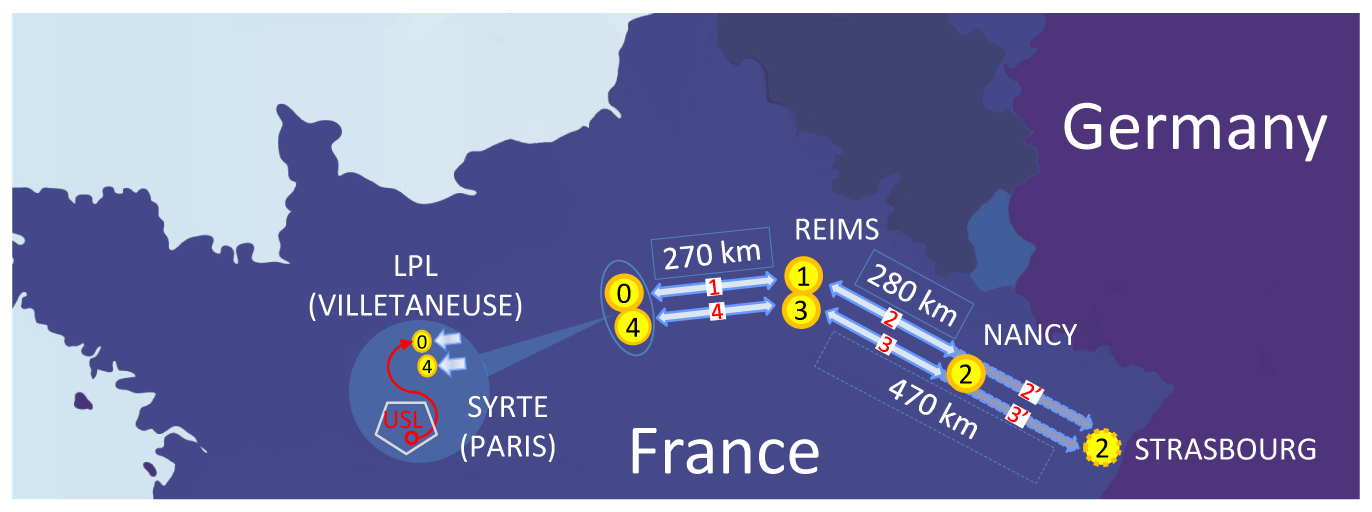
\includegraphics[width=0.6\textwidth,keepaspectratio]{Images/SYRTE_Link_Map.jpg}
    \end{block}

    \begin{block}{Schematic of Cascaded Optical Fiber Link}
        \centering
        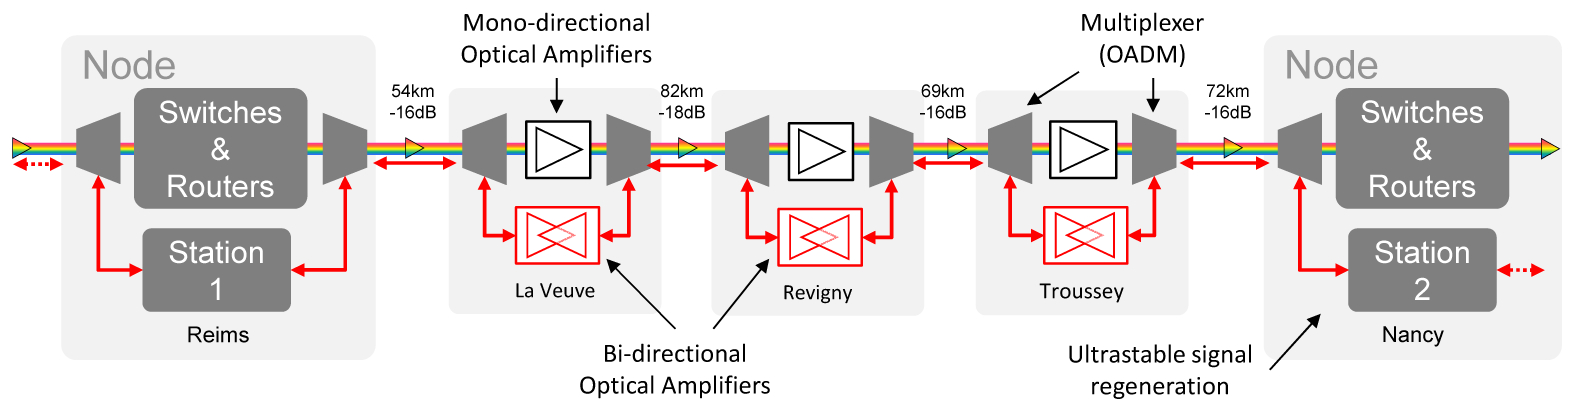
\includegraphics[width=0.8\textwidth,keepaspectratio]{Images/SYRTE_Link_Schem.jpg}
    \end{block}

    \cite{Chiodo2015}
\end{frame}

\begin{frame}\frametitle{Repeater Station}
    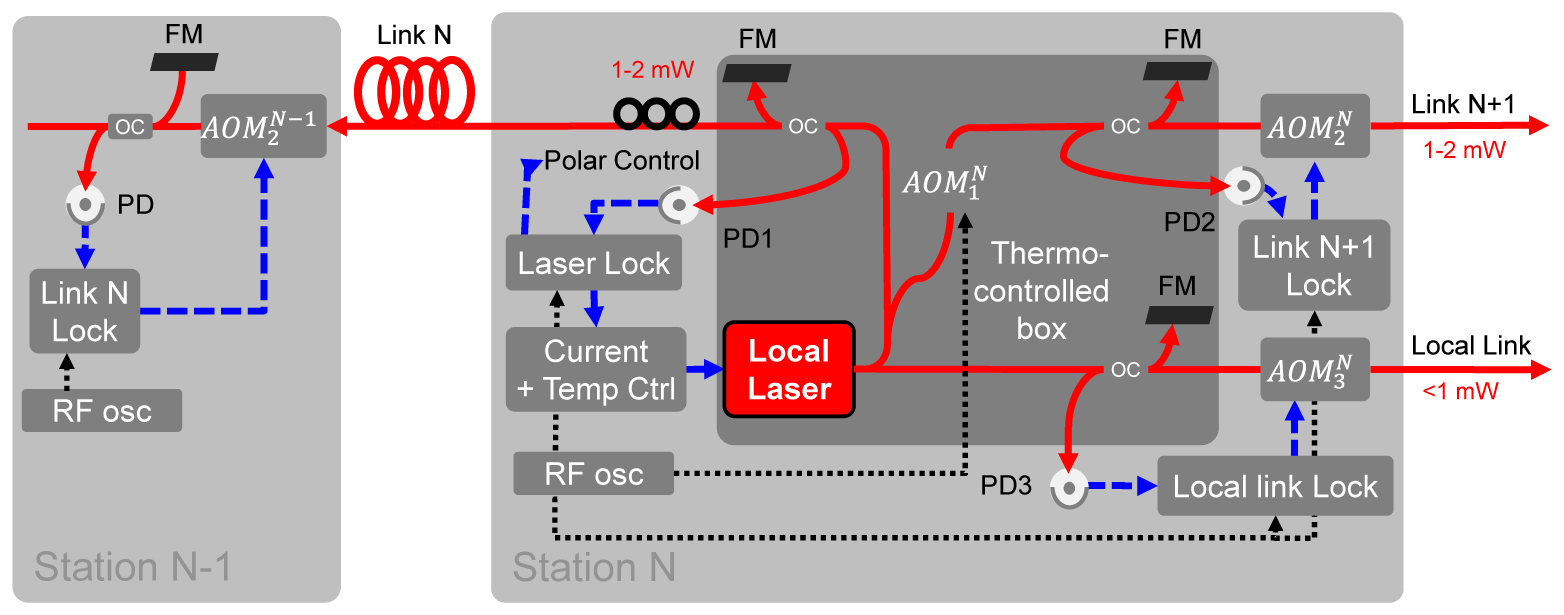
\includegraphics[width=1.0\textwidth,keepaspectratio]{Images/Repeater_Schem.jpg}
   
    \cite{Chiodo2015}
\end{frame}

\section{Results} 
\begin{frame}\frametitle{Experimental Uncertainties}
    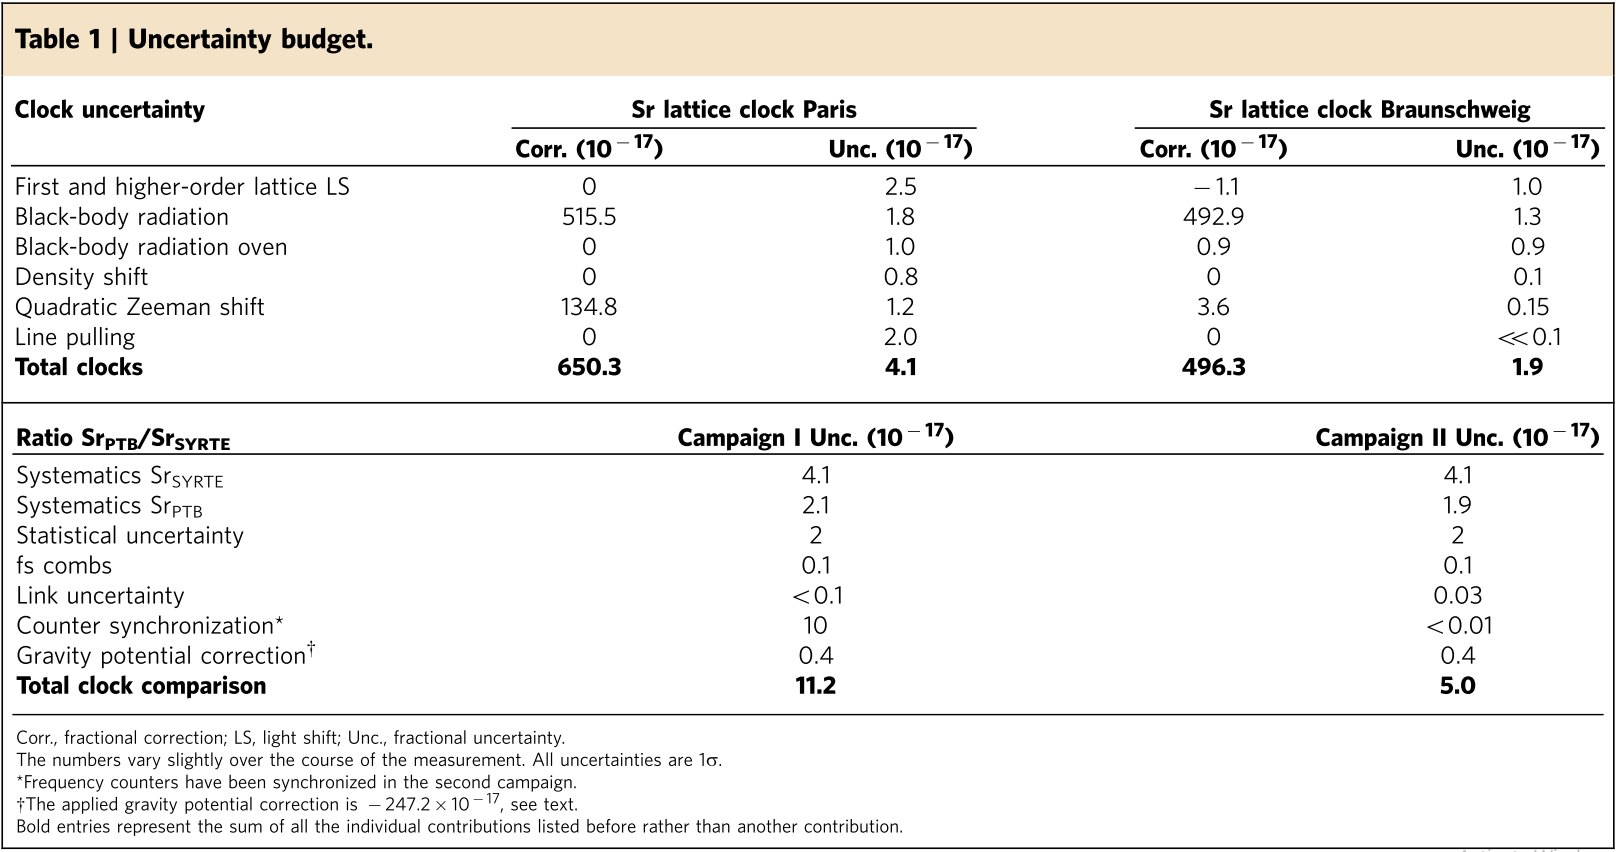
\includegraphics[width=1.0\textwidth,keepaspectratio]{Images/Uncert_Table.png}

    \cite{Lisdat2016}
\end{frame}

\begin{frame}\frametitle{Frequency Ratio Between PTB and SYRTE}
    \begin{center} 
        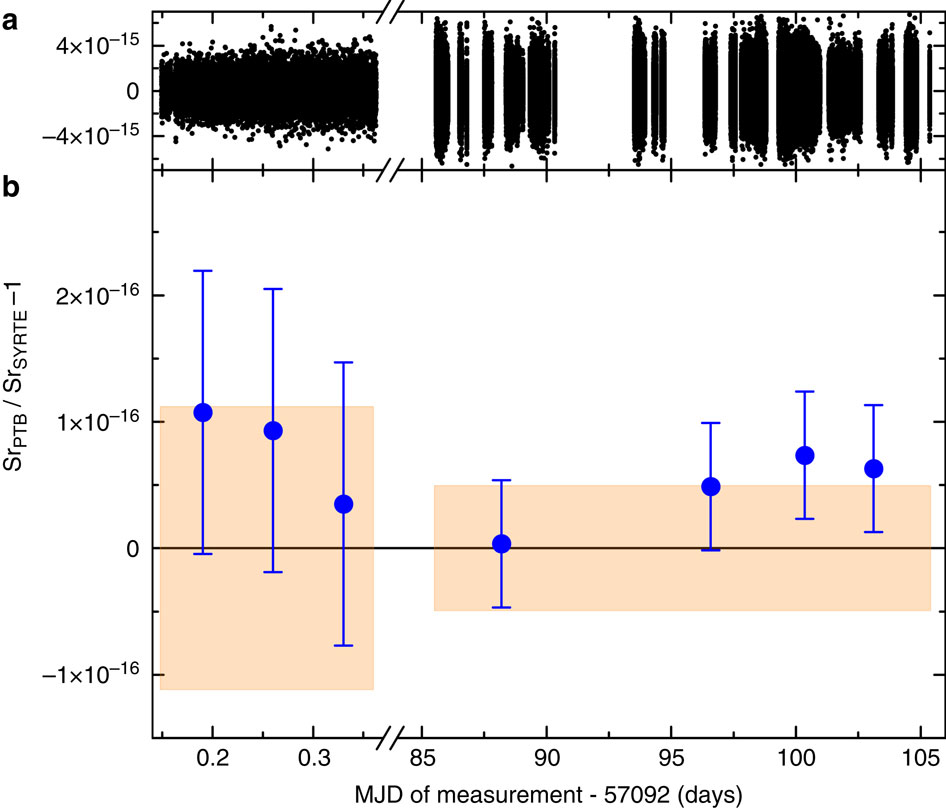
\includegraphics[width=0.7\textwidth,keepaspectratio]{Images/Freq_Ratio.jpg}
    \end{center} 

    \cite{Lisdat2016}
\end{frame}

\begin{frame}\frametitle{Allen Deviation Plots}
    \begin{center}
        \cite{Lisdat2016}
        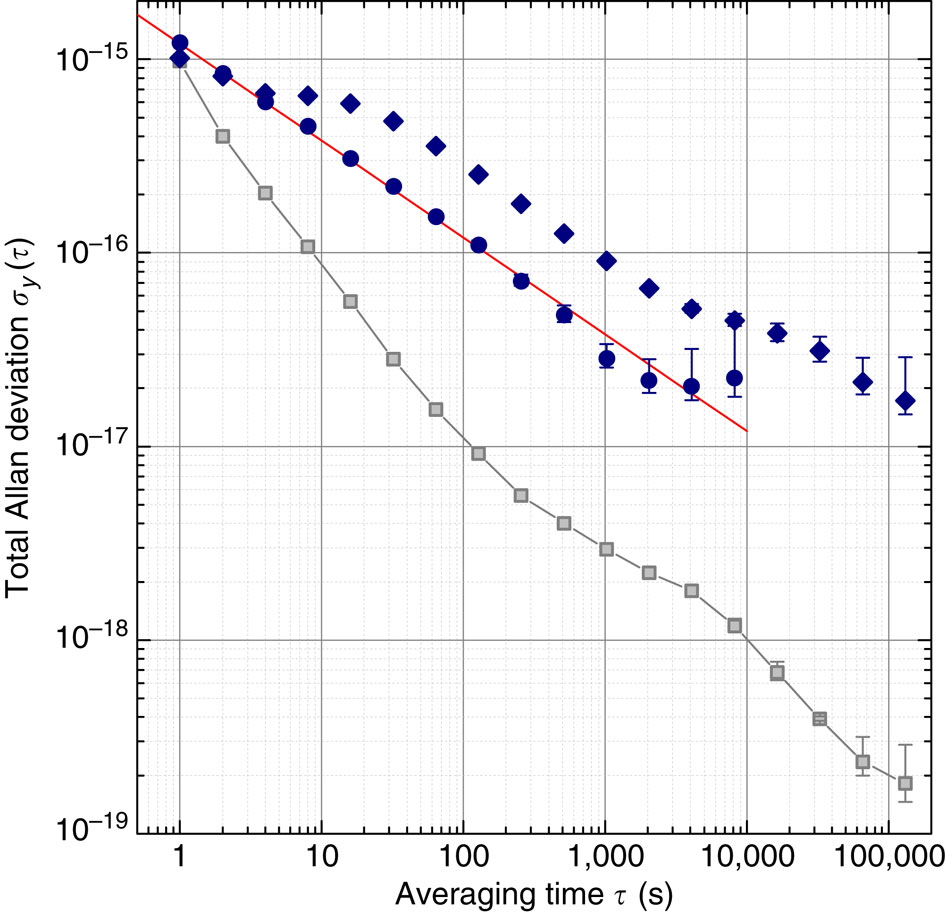
\includegraphics[width=0.65\textwidth,keepaspectratio]{Images/Allen_Dev.jpg}
    \end{center}

\end{frame}

\section{Conclusion} 
\begin{frame}\frametitle{Conclusions}  
    \begin{itemize}
        \item Researchers measured a fractional offset between the two clocks as $(4.7\pm5.0)\times10^{-17}$.
        \item After less than an hour of averaging they reached a statistical uncertainty of $2\times10^{-17}$. This marks an order of magnitude improvement on all previous long distance frequency comparisons with a four order of magnitude reduction in measurement time.
        \item The foundations are set for an optical clock network across the continent of Europe.
    \end{itemize}
\end{frame}

\begin{frame}{Further Reading}
    \tiny
    \bibliographystyle{abbrvnat}
    \bibliography{References}
\end{frame}

\end{document}

